\documentclass[11pt]{article}
\usepackage{amsmath, amssymb, amscd, amsthm, amsfonts}
\usepackage{graphicx}
\usepackage{hyperref}
\hypersetup{
    colorlinks=true,
    linkcolor=blue,
    filecolor=magenta,      
    urlcolor=cyan,
    pdftitle={Overleaf Example},
    pdfpagemode=FullScreen,
    }
\usepackage[dvipsnames]{xcolor}

\oddsidemargin 0pt
\evensidemargin 0pt
\marginparwidth 40pt
\marginparsep 10pt
\topmargin -20pt
\headsep 10pt
\textheight 8.7in
\textwidth 6.65in
\linespread{1.2}

\title{Course Report: Classification}
\author{Nan He}
\date{}

\newtheorem{theorem}{Theorem}
\newtheorem{lemma}[theorem]{Lemma}
\newtheorem{conjecture}[theorem]{Conjecture}

\newcommand{\rr}{\mathbb{R}}

\newcommand{\al}{\alpha}
\DeclareMathOperator{\conv}{conv}
\DeclareMathOperator{\aff}{aff}

\begin{document}

\maketitle

%\begin{abstract}
%(Abs)
%\end{abstract}

\section{Main objective of the analysis}\label{section-introduction-1}
Acknowledgement: this is a course project for \href{https://www.coursera.org/professional-certificates/ibm-machine-learning}{IBM Machine Learning professional certificate}. The project notebook can be accessed \href{https://github.com/henankf223/Assignment-2/blob/26433c172a58e934f1039ef8de647232f05e747c/PES_DVR_pd.ipynb}{here}.

The data I will be using is a heart failure prediction dataset from Kaggle, the link for the data set is \href{https://www.kaggle.com/fedesoriano/heart-failure-prediction}{here}.
The goal of this report is to find a model that predict possible heart failure.
I will clean the data, and use three different classification method to build the model.
The hyperparameters of each model will be benchmarked using cross-validation.
The model will be tested on the hold out set, using accuracy, F1 score, and ROC curve as metrics.

\section{Description of the data set}\label{section-introduction-2}
The data set includes 11 clinical features for predicting heart disease events and 918 labels in total.
The categorical features are "Sex", "ChestPainType", "FastingBS", "RestingECG", "ExerciseAngina", and "ST\textunderscore Slope", of which "Sex", "FastingBS", and "ExerciseAngina" are binary.
The numerical features are "Age", "RestingBP", "Cholesterol", "MaxHR", and "Oldpeak".
The target is "HeartDisease", which is a binary feature, indicating the occurance of the heart disease event.
Example data looks like:

\begin{figure}[h]
\centerline{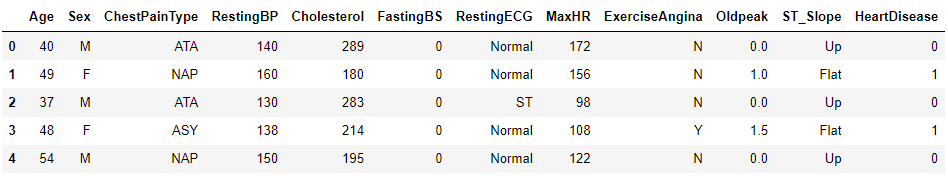
\includegraphics[scale=0.5]{cls1.png}}
\caption{Example data before cleaning.}
\end{figure}

\section{Data exploration, cleaning, and feature engineering}\label{section-introduction-3}
The description of the data is:

\begin{figure}[h]
\centerline{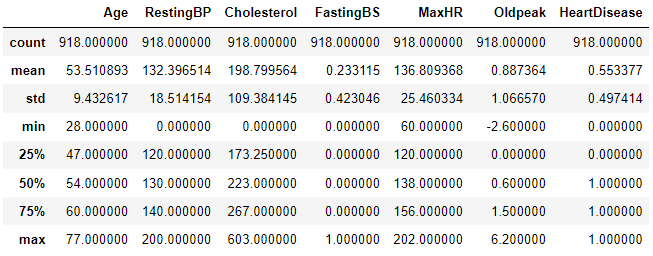
\includegraphics[scale=0.6]{cls2.png}}
\caption{Data descriptions.}
\end{figure}

I firstly check whether there is any empty data, and find none.
The pairplot of all numerical data is shown, which show good predictability.

\begin{figure}[h!]
\centerline{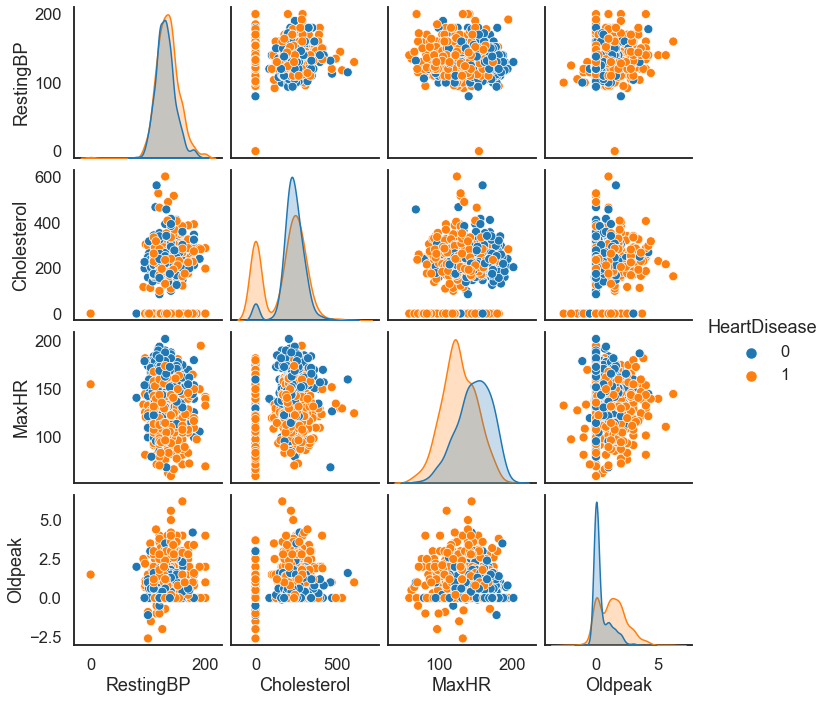
\includegraphics[scale=0.5]{cls3.png}}
\caption{Pairplot of all numerical data.}
\end{figure}

The next step is to encode the categorical data, since we are going to use some models that requires numerical inputs.
For binary data "Sex", "FastingBS", and "ExerciseAngina", I encode them as 0 and 1 in place; while for "ChestPainType", "RestingECG", and "ST\textunderscore Slope", I do one-hot encoding. The number of features after encoding is 17.

The next step is to check whether the data is balances, to decide whether we need to upsample or downsample after the train-test split. The target "HeartDisease" has 508 "1" and 410 "0", which is fairly balanced; thus no need for using resample methods.

Before running the model, we split the data into a train set and a test set, holding 25\% of data out of the model training procedure. The labels in the training set is 688.
The numerical features are then scaled using standard scalar. This step eliminate the bias in algorithms based on distances.
The data is now ready to train.

\section{Testing different models}\label{section-model}
The first model I tested is a simple \textbf{logistic regression} with L2 regularization.
The second model is a \textbf{SVM classifier} with different kernels and regularizations.
The third model is a \textbf{Random Forest classifier} with various criterion and max features for tree split.

To tune the model hyperparameter, the grid search cross-validation is performed on regularization parameter "C" for all model.
For SVM classifier, the kernel type (linear, polynomial, radial basis functions, sigmoid) and the gamma value of the gaussian functions are tuned.
For Ramdom Forest classifier, the tree-split criterion (Gini, entropy), the max features for each split, and the number of estimators are tuned.

After cross-validation, all model are tested on the test set, the results are shown in various metrics:

\begin{table}[h!]
\caption{Results for all three models on the test set, LR stands for Logistic regression, SVC for SVM classifier, RFC for Random Forest classifier.}
\begin{tabular}{llllllll}
\hline
\hline
Model & True  & True & False & False &  &   & \\
Name & Positive & Negative & Negative & Positive & Accuracy & F1 score & ROC AUC \\
\hline
LR & 112 & 86 & 20 & 12 & 0.861 & 0.875 & 0.937 \\
SVC & 112 & 87 & 20 & 11 & 0.865 & 0.878 & 0.932 \\
RFC & 117 & 88 & 15 & 10 & 0.891 & 0.903 & 0.945 \\
\hline
\hline
\end{tabular}
\end{table}

The ROC curves for all three models are:

\begin{figure}[h!]
\centerline{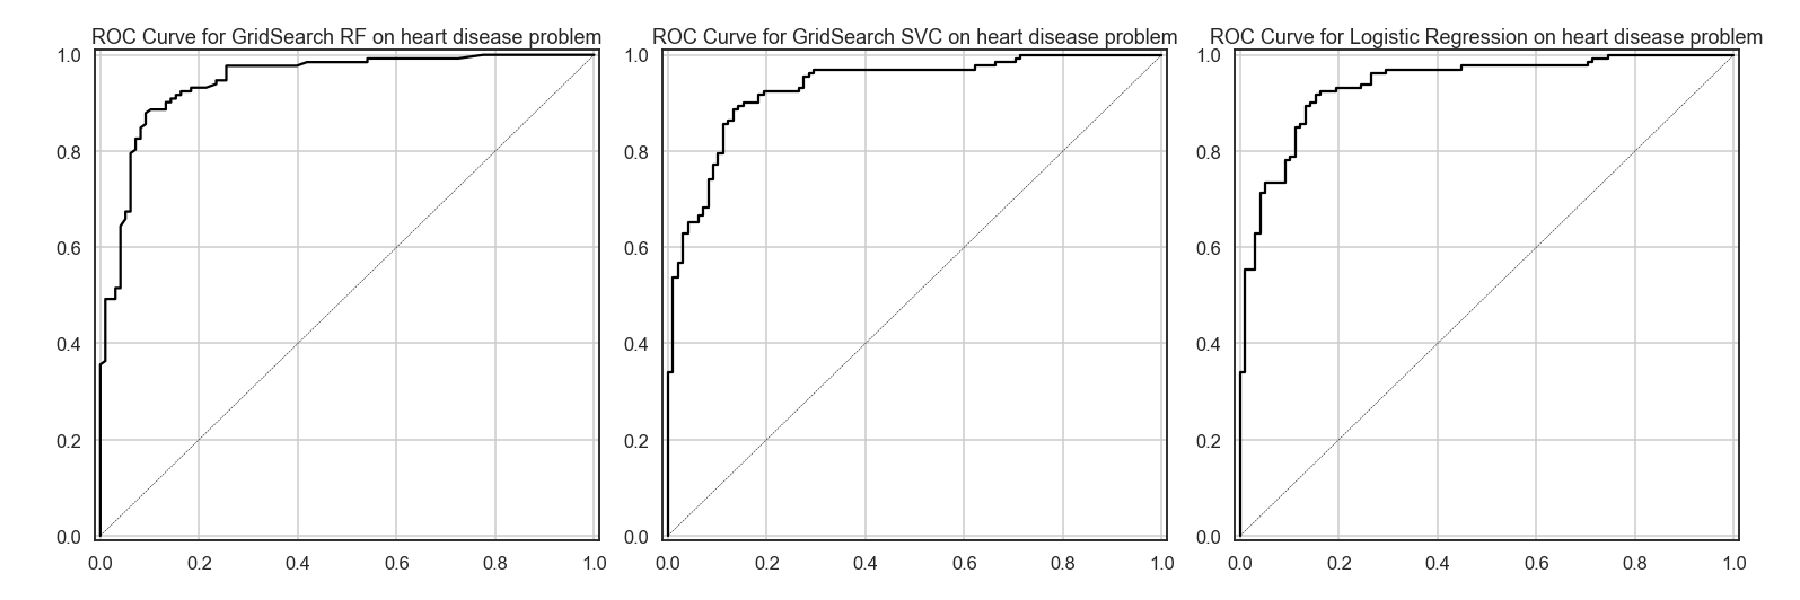
\includegraphics[scale=0.6]{cls_fi.pdf}}
\caption{ROC curve for LR, SVC, and RFC models.}
\end{figure}

\section{Final model choices and analysis}\label{section-pred}
From the results, the Random forest model with hyper-parameter tuned performs best on the test set.
The hyperparameter for the model is: \\
Criterion: Gini, Max features: 2, Estimators: 200.
However, the Random forest model tooks the longest time to train and tune, while logistic regression and Support Vector Machine are much faster.
If the data set is larger, the hyper-parameter tuning of Random forest could be difficult.

\section{Key Findings and Insights}\label{section-find}
One of the major finding is that the grid-search cross-validation is vital for Support Vector Machine classifiers and ensemble methods like Random forest classifiers.
For example, if I simply use SVC with radial basis function, gamma$=1.0$ and $C=10.0$, the accuracy on the test set will be only 0.748, and produce 50 false positive, much worse than simple logistic regression.
Therefore, to use SVC and RFC, the cross-validation procedure is very important and cannot be skipped.

\section{Summary and suggestions for next steps}\label{section-sugg}
In summary, this report provide a tuned model to predict heart-failure events, with 0.891 accuracy.
The possible next step is to further tun the hyper-parameters, and try more models.
Another possible direction is to consider ignoring unimportant features.

%\bibliographystyle{alpha}
%\bibliography{references} % see references.bib for bibliography management

\end{document}
